\documentclass[a4paper]{article}

\usepackage{float}

% Need to define the build/ dir as the output dir of the package
\usepackage[outputdir=build]{minted}
\usemintedstyle{tango}

% To use greek
\usepackage{fontspec}
\usepackage{polyglossia}
\setmainfont[]{DejaVu Serif}

% Package for captions
% Set spacing between caption and figure or table
\usepackage{caption}
\captionsetup[table]{skip=10pt}
\captionsetup[figure]{skip=15pt}

\usepackage[hidelinks,unicode]{hyperref}
\usepackage[capitalise,noabbrev]{cleveref}
\usepackage[backend=biber]{biblatex}
\addbibresource{references.bib}

\renewcommand\listoflistingscaption{List of source codes}
\renewcommand{\listfigurename}{List of plots}
\renewcommand{\listtablename}{Tables}


\begin{document}

\tableofcontents

\listoffigures

\listoflistings

\listoftables

\newpage

\section{First Article Section}
\paragraph{}Lorem ipsum dolor sit amet, consectetur adipiscing elit, sed do eiusmod tempor incididunt ut labore et dolore magna aliqua.
Ut enim ad minim veniam, quis nostrud exercitation ullamco laboris nisi ut aliquip ex ea commodo consequat. Duis aute irure dolor in
reprehenderit in voluptate velit esse cillum dolore eu fugiat nulla pariatur. Excepteur sint occaecat cupidatat non proident, sunt in
culpa qui officia deserunt mollit anim id est laborum.
\paragraph{}Το Lorem Ipsum είναι απλά ένα κείμενο χωρίς νόημα για τους επαγγελματίες της τυπογραφίας και στοιχειοθεσίας.
Το Lorem Ipsum είναι το επαγγελματικό πρότυπο όσον αφορά το κείμενο χωρίς νόημα, από τον 15ο αιώνα, όταν ένας ανώνυμος
τυπογράφος πήρε ένα δοκίμιο και ανακάτεψε τις λέξεις για να δημιουργήσει ένα δείγμα βιβλίου. Όχι μόνο επιβίωσε πέντε αιώνες,
αλλά κυριάρχησε στην ηλεκτρονική στοιχειοθεσία, παραμένοντας με κάθε τρόπο αναλλοίωτο. Έγινε δημοφιλές τη δεκαετία του '60 με την
έκδοση των δειγμάτων της Letraset όπου περιελάμβαναν αποσπάσματα του Lorem Ipsum, και πιο πρόσφατα με το λογισμικό ηλεκτρονικής
σελιδοποίησης όπως το Aldus PageMaker που περιείχαν εκδοχές του Lorem Ipsum.

\begin{itemize}
\item This is the first item, of itemize
\item This is the second item, of itemize
\end{itemize}

% With the star the number in the section is omitted
\section*{Subsection without numbering, asterisk}

\begin{enumerate}
\item This is the first item, of enumerate
\item This is the second item, of enumerate
\end{enumerate}

% It creates a nice aesthetic to start a new chapter/section in a new page
\newpage


\section{Second Article Section}
\paragraph{}
sed quia non numquam eius modi tempora incidunt ut labore et dolore magnam aliquam quaerat voluptatem. Ut enim ad minima
veniam, quis nostrum exercitationem ullam corporis suscipit laboriosam, nisi ut aliquid ex ea commodi

\begin{figure}[b!]
\centering
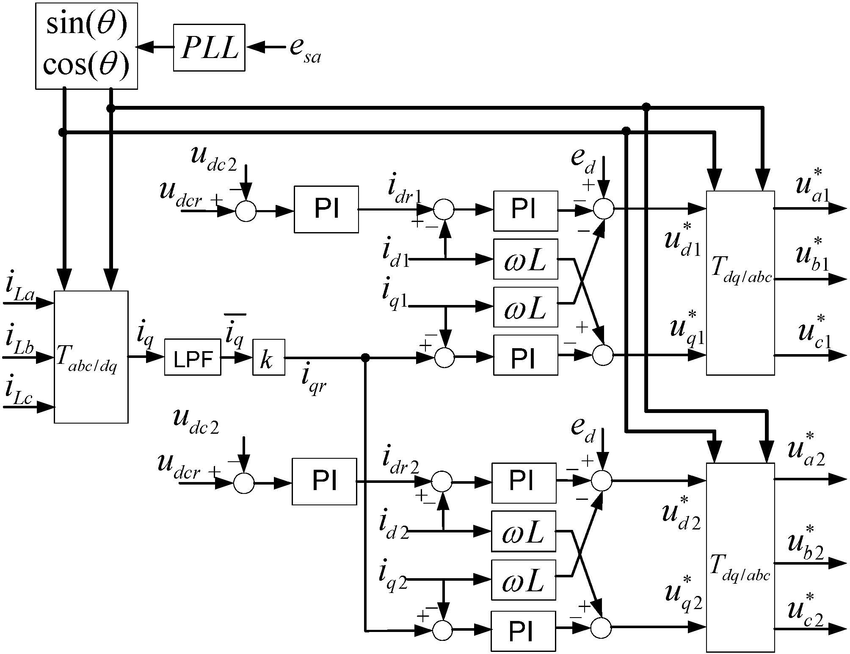
\includegraphics[scale=0.3]{assets/figures/figure_1.png}
\caption{This is the caption of the first figure}
\label{fig:figure 1}
\end{figure}

\subsection{This is a subsection}
\paragraph{}
Lorem ipsum dolor sit amet, consectetur adipiscing elit, sed do eiusmod tempor incididunt ut labore et dolore magna aliqua.
Ut enim ad minim veniam, quis nostrud exercitation ullamco laboris nisi ut aliquip ex ea commodo consequat. Duis aute irure
dolor in reprehenderit in voluptate velit esse cillum dolore eu fugiat nulla pariatur. Excepteur sint occaecat cupidatat
non proident, sunt in culpa qui officia deserunt mollit anim id est laborum.

\subsection{This is a subsection}
\paragraph{}
Sed ut perspiciatis unde omnis iste natus error sit voluptatem accusantium doloremque laudantium, totam rem aperiam,
eaque ipsa quae ab illo inventore veritatis et quasi architecto beatae vitae dicta sunt explicabo. Nemo enim ipsam
voluptatem quia voluptas sit aspernatur aut odit aut fugit, sed quia consequuntur magni dolores eos qui ratione
voluptatem sequi nesciunt. Neque porro quisquam est, qui dolorem ipsum quia dolor sit amet, consectetur, adipisci
velit, consequatur? Quis autem vel eum iure reprehenderit qui in ea voluptate velit esse quam nihil molestiae
consequatur, vel illum qui dolorem eum fugiat quo voluptas nulla pariatur?

\begin{table}[h!]
\centering
\caption{Fisher's Iris data}
\label{tab:table1}

% This is to resize the table to fit the page
\resizebox{\linewidth}{!}{%
% With l,c,r you define the alignment of each column
\begin{tabular}{l||c|c|c|c|r}
    Dataset Order & Sepal Length & Sepal Width & Petal Length & Petal Length & Species\\
    \hline
    1 &	5.1 & 3.5 & 1.4 & 0.2 & I. setosa\\
    2 &	4.9 & 3.0 & 1.4 & 0.2 & I. setosa\\
    3 &	4.7 & 3.2 & 1.3 & 0.2 & I. setosa\\
    4 &	4.6 & 3.1 & 1.5 & 0.2 & I. setosa\\
\end{tabular}
}
\end{table}

\subsection*{This is a subsection without numbering}
\paragraph{}
At vero eos et accusamus et iusto odio dignissimos ducimus qui blanditiis praesentium voluptatum deleniti atque
corrupti quos dolores et quas molestias excepturi sint occaecati cupiditate non provident, similique sunt in culpa
qui officia deserunt mollitia animi, id est laborum et dolorum fuga. Et harum quidem rerum facilis est et expedita
distinctio. Nam libero tempore, cum soluta nobis est eligendi optio cumque nihil impedit quo minus id quod maxime
placeat facere possimus, omnis voluptas assumenda est, omnis dolor repellendus. Temporibus autem quibusdam et aut
officiis debitis aut rerum necessitatibus saepe eveniet ut et voluptates repudiandae sint et molestiae non recusandae.
Itaque earum rerum hic tenetur a sapiente delectus, ut aut reiciendis voluptatibus maiores alias consequatur aut
perferendis doloribus asperiores repellat.

\begin{figure}[H]
\centering
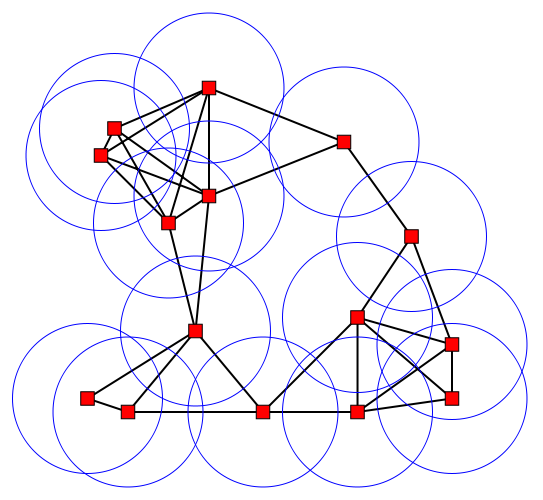
\includegraphics[width=\linewidth]{assets/figures/figure_2.png}
\caption{This is the caption of the second figure}
\label{fig:figure 2}
\end{figure}

% It creates a nice aesthetic to start a new chapter/section in a new page
\newpage


\section{This is a section containing code}
\paragraph{}
At vero eos et accusamus et iusto odio dignissimos ducimus qui blanditiis praesentium voluptatum deleniti atque
corrupti quos dolores et quas molestias excepturi sint occaecati cupiditate non provident, similique sunt 

\begin{listing}[ht]
\caption{Python code example}
\label{listing:python example}

\begin{minted}{python}
import numpy as np
    
def incmatrix(genl1,genl2):
    m = len(genl1)
    n = len(genl2)
    M = None #to become the incidence matrix
    VT = np.zeros((n*m,1), int)  #dummy variable
    
    #compute the bitwise xor matrix
    M1 = bitxormatrix(genl1)
    M2 = np.triu(bitxormatrix(genl2),1) 
    
    for i in range(m-1):
        for j in range(i+1, m):
            [r,c] = np.where(M2 == M1[i,j])
            for k in range(len(r)):
                VT[(i)*n + r[k]] = 1;
                VT[(i)*n + c[k]] = 1;
                VT[(j)*n + r[k]] = 1;
                VT[(j)*n + c[k]] = 1;
    
                if M is None:
                    M = np.copy(VT)
                else:
                    M = np.concatenate((M, VT), 1)
    
                VT = np.zeros((n*m,1), int)
    
    return M
\end{minted}
\end{listing}

\end{document}